\documentclass[aspectratio=169]{beamer}
\usetheme{Boadilla}
\usecolortheme{default}
\usepackage[utf8]{inputenc}
% \usepackage{ngerman}
\usepackage{booktabs}
\usepackage{color}
% Fonts
% https://tug.org/FontCatalogue/
% https://ctan.org/pkg/free-math-font-survey

% fontenc – Standard package for selecting font encodings
% https://ctan.org/pkg/fontenc
\usepackage[T1]{fontenc}

\usepackage{comment}
\usepackage{textpos}
\usepackage{textgreek}
\usepackage{graphicx}
% Serif font
\usepackage{bera}

% Mono font
\usepackage{nimbusmononarrow}

% Sans-Serif font (fallback)
% tgheros
\usepackage{tgheros}

% Font Roboto Condensed
% https://tug.org/FontCatalogue/robotocondensed/
% https://ctan.org/pkg/roboto
\usepackage[sfdefault,condensed]{roboto}

% Fancy verbatim text for setting code inline
\usepackage{fancyvrb}
\usepackage{verbatimbox}

% Tikz based on a template by Aidan Hogan
\usepackage{tikz}
\usetikzlibrary{shapes.geometric, trees,arrows, arrows.meta}
\usepackage{kg-macros}

\usepackage{relsize}

% Highlights in text
\newcommand{\myblue}[1]{{\color{blue}{#1}}}
\newcommand{\myred}[1]{{\color{red}{#1}}}
\definecolor{emerald}{rgb}{0.31, 0.78, 0.47}
\newcommand{\mygreen}[1]{{\color{emerald}{#1}}}


% Turtle box / SPARQL box listing
\definecolor{olivegreen}{rgb}{0.2,0.8,0.5}
\definecolor{grey}{rgb}{0.5,0.5,0.5}
\definecolor{htmlgreen}{HTML}{E8F0E8}
\definecolor{htmlblue}{HTML}{f7f8ff}

\usepackage{listings}
\lstdefinelanguage{ttl}{
sensitive=true,
morecomment=[l][\color{grey}]{@},
morecomment=[l][\color{olivegreen}]{\#},
keywordstyle=\color{cyan},
morekeywords={xmlns,version,owl,rdf,rdfs,xml,xsd},
backgroundcolor=\color{htmlgreen},
frame=single,
basicstyle=\footnotesize\ttfamily
}
\lstdefinelanguage{SPARQL}{
sensitive=true,
morecomment=[l][\color{grey}]{@},
morecomment=[l][\color{olivegreen}]{\#},
keywordstyle=\color{cyan},
morekeywords={SELECT,FROM,WHERE,FILTER,PREFIX,ORDER BY,GROUP BY,HAVING,LIMIT,OFFSET},
backgroundcolor=\color{htmlblue},
frame=single,
basicstyle=\footnotesize\ttfamily
}
\definecolor{maroon}{rgb}{0.5,0,0}
\definecolor{darkgreen}{rgb}{0,0.5,0}

\lstdefinelanguage{TURTLE}
{
	%basicstyle=\ttfamily,
	morestring=[b]",
	moredelim=[s][\bfseries\color{maroon}]{<}{\ },
	moredelim=[s][\bfseries\color{maroon}]{</}{>},
	moredelim=[l][\bfseries\color{maroon}]{/>},
	moredelim=[l][\bfseries\color{maroon}]{>},
	morecomment=[s]{<?}{?>},
	morecomment=[s]{<!--}{-->},
	moredelim=[s][\bfseries\color{black}]{\:}{\ },
	commentstyle=\color{green},
	stringstyle=\color{blue},
	identifierstyle=\color{darkgreen},
	morekeywords={@prefix}% list your attributes her
}

\definecolor{gray}{rgb}{0.4,0.4,0.4}
\definecolor{darkblue}{rgb}{0.0,0.0,0.6}
\definecolor{cyan}{rgb}{0.0,0.6,0.6}
\lstdefinelanguage{XML}
{
	morestring=[b]",
	morestring=[s]{>}{<},
	morecomment=[s]{<?}{?>},
	stringstyle=\color{black},
	identifierstyle=\color{darkblue},
	keywordstyle=\color{cyan},
	morekeywords={xmlns,version,type}% list your attributes here
}
\lstset{literate=%
  {Ö}{{\"O}}1
  {Ä}{{\"A}}1
  {Ü}{{\"U}}1
  {ß}{{\ss}}1
  {ü}{{\"u}}1
  {ä}{{\"a}}1
  {ö}{{\"o}}1
}

\colorlet{punct}{red!60!black}
\definecolor{background}{HTML}{EEEEEE}
\definecolor{delim}{RGB}{20,105,176}
\colorlet{numb}{magenta!60!black}

\lstdefinelanguage{json}{
    basicstyle=\normalfont\ttfamily,
    numbers=left,
    numberstyle=\scriptsize,
    stepnumber=1,
    numbersep=8pt,
    showstringspaces=false,
    breaklines=true,
    frame=lines,
    backgroundcolor=\color{background},
    literate=
     *{0}{{{\color{numb}0}}}{1}
      {1}{{{\color{numb}1}}}{1}
      {2}{{{\color{numb}2}}}{1}
      {3}{{{\color{numb}3}}}{1}
      {4}{{{\color{numb}4}}}{1}
      {5}{{{\color{numb}5}}}{1}
      {6}{{{\color{numb}6}}}{1}
      {7}{{{\color{numb}7}}}{1}
      {8}{{{\color{numb}8}}}{1}
      {9}{{{\color{numb}9}}}{1}
      {:}{{{\color{punct}{:}}}}{1}
      {,}{{{\color{punct}{,}}}}{1}
      {\{}{{{\color{delim}{\{}}}}{1}
      {\}}{{{\color{delim}{\}}}}}{1}
      {[}{{{\color{delim}{[}}}}{1}
      {]}{{{\color{delim}{]}}}}{1},
}

\graphicspath{{lecture/images/}{lecture/open_images/}}



\title[Ontologies]{RDF-star and SPARQL-star}  

\author[]{Prof. Dr. Ricardo Usbeck and Longquan Jiang\\
\url{https://github.com/semantic-systems/rdf-star-tutorial}} 
\date{}


\begin{document}

\begin{frame}
\titlepage
\end{frame}

\begin{frame}{Overview}{\quad}
\tableofcontents
\end{frame}

\section{Background and Motivation}
\begin{frame}{Background and Motivation}
    \begin{itemize}
        \item The RDF data model allows you to state world facts as three-part (subject, predicate, object) triples.
        \begin{itemize}
            \item Predicate of a triple is a property specified with an IRI
            \item Subject of a triple and object can each be an IRI referencing any entity, and the object can also be a literal value, dates, numbers, or boolean values
        \end{itemize}
        \item Example: "employee38 has the familyName Smith" $\rightarrow$ (employee38, familyName, "Smith")
    \end{itemize}
    \begin{figure}
        \centering
        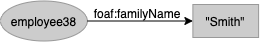
\includegraphics[scale=0.5]{images/Example-1.png}
        %\caption{Example 1}
        %\label{fig:my_label}
    \end{figure}
\end{frame}

\begin{frame}{Background and Motivation}
    \begin{itemize}
        \item Sometimes, we want the subject or object of a triple to refer to another triple
        \item Example: "according to employee22, employee38 has a jobTitle of Assistant Designer"
    \end{itemize}
    \begin{figure}
        \centering
        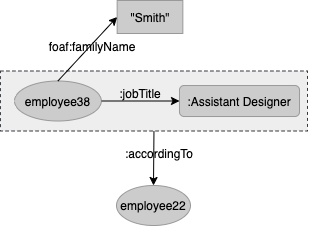
\includegraphics[scale=0.5]{images/Example-2.png}
        %\caption{Example 2}
        %\label{fig:my_label}
    \end{figure}
\end{frame}

\begin{frame}{Background and Motivation}
    \begin{itemize}
        \item Existing approaches:
        \begin{itemize}
            \item \textbf{Standard Reification} (RDF 1.0, 1999)
        \end{itemize}
    \end{itemize}
    \begin{figure}
        \centering
        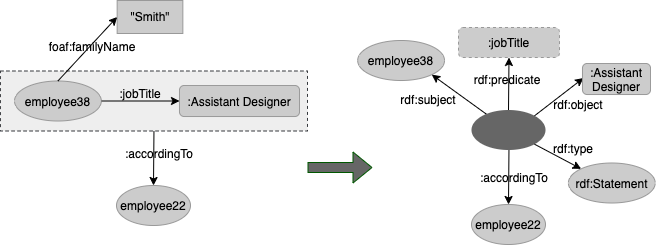
\includegraphics[scale=0.5]{images/Example-2-To-Reification.png}
    \end{figure}
\end{frame}

\begin{frame}[fragile]{Background and Motivation}
    \begin{itemize}
        \item Existing approaches:
            \begin{itemize}
                \item \textbf{Standard Reification} (RDF 1.0, 1999)
            \end{itemize}
    \end{itemize}
    \begin{minipage}{0.56\textwidth}
    \small{Who has a JobTitle of Assistant Designer according to whom?}
\begin{lstlisting}[language=SPARQL]
PREFIX ...
SELECT ?who ?whom WHERE {
 ?claim rdf:type rdf:Statement .
 ?claim rdf:subject ?who .
 ?claim rdf:predicate :jobTitle .
 ?claim rdf:object :AssistantDesigner .
 ?claim :accordingTo ?whom .
}
\end{lstlisting}
\end{minipage}
\begin{minipage}{0.43\textwidth}
\centering
	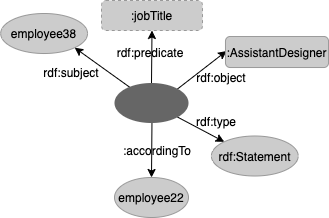
\includegraphics[scale=0.5]{images/Example-2-Reification.png}
\end{minipage}
\end{frame}

\begin{frame}{Background and Motivation}
    \begin{itemize}
        \item Existing approaches:
            \begin{itemize}
                \item Standard Reification (RDF 1.0, 1999)
                \item \textbf{Single-triple Named Graphs} (Carroll et al., 2005; RDF 1.1, 2014)
            \end{itemize}
    \end{itemize}
    \begin{figure}
        \centering
        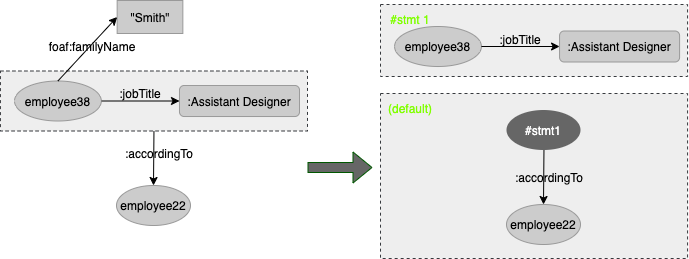
\includegraphics[scale=0.6]{images/Example-2-To-NamedGraph.png}
    \end{figure}
\end{frame}

\begin{frame}[fragile]{Background and Motivation}
    \begin{itemize}
        \item Existing approaches:
            \begin{itemize}
                \item Standard Reification (RDF 1.0, 1999)
                \item \textbf{Single-triple Named Graphs} (Carroll et al., 2005; RDF 1.1, 2014)
            \end{itemize}
    \end{itemize}
        \begin{minipage}{0.56\textwidth}
    \small{Who has a JobTitle of Assistant Designer according to whom?}
\begin{lstlisting}[language=SPARQL]
PREFIX ...
SELECT ?who ?whom WHERE {
 GRAPH ?claim {
  ?who :jobTitle :AssistantDesigner .
 }
 ?claim :accordingTo ?whom .
}
\end{lstlisting}
\end{minipage}
\begin{minipage}{0.43\textwidth}
\centering
	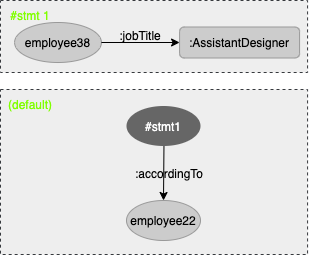
\includegraphics[scale=0.5]{images/Example-2-NamedGraph.png}
\end{minipage}
\end{frame}

\begin{frame}{Background and Motivation}
    \begin{itemize}
        \item Existing approaches:
            \begin{itemize}
                \item Standard Reification (RDF 1.0, 1999)
                \item Single-triple Named Graphs (Carroll et al., 2005; RDF 1.1, 2014)
                \item \textbf{Singleton Properties} (Nguyen et al., 2014)
            \end{itemize}
    \end{itemize}
    \begin{figure}
        \centering
        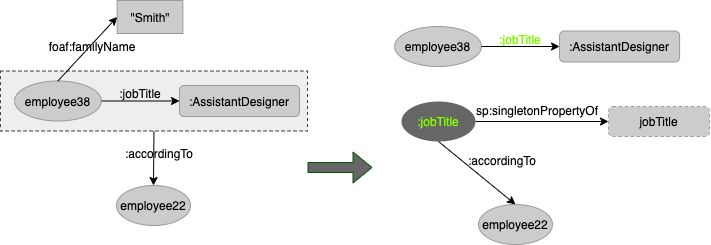
\includegraphics[scale=0.5]{images/Example-2-To-SingletonProperties.png}
    \end{figure}
\end{frame}

\begin{frame}[fragile]{Background and Motivation}
    \begin{itemize}
        \item Existing approaches:
            \begin{itemize}
                \item Standard Reification (RDF 1.0, 1999)
                \item Single-triple Named Graphs (Carroll et al., 2005; RDF 1.1, 2014)
                \item \textbf{Singleton Properties} (Nguyen et al., 2014)
            \end{itemize}
    \end{itemize}
    
    \begin{minipage}{0.56\textwidth}
    \smaller{Who has a JobTitle of Assistant Designer according to whom?}
\begin{lstlisting}[language=SPARQL]
PREFIX ...
SELECT ?who ?whom WHERE {
    ?who ?claim :AssistantDesigner .
    ?claim sp:singletonPropertyOf :jobTitle .
    ?claim :accordingTo ?whom .
}
\end{lstlisting}
\end{minipage}
\begin{minipage}{0.43\textwidth}
\centering
	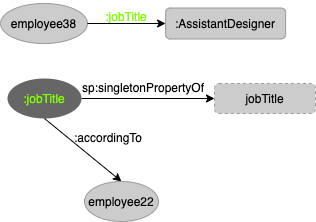
\includegraphics[scale=0.5]{images/Example-2-SingletonProperties.png}
\end{minipage}
\end{frame}

\begin{frame}{Background and Motivation}
    \begin{itemize}
        \item However, it is \textbf{complicated} and \textbf{cumbersome} to express metadata about triples in RDF or query it with SPARQL
        \item Summary of Existing Approaches:
        \begin{itemize}
            \item Standard Reification
                \begin{itemize}
                    \item Pros: Standard
                    \item Cons: Verbose; Incomplete/overloaded reified statements
                \end{itemize}
            \item Single-triple Named Graphs
                \begin{itemize}
                    \item Pros: Standard
                    \item Cons: Unspecified semantics; Clutters datasets with "artificial" named graphs
                \end{itemize}
            \item Singleton Properties
                \begin{itemize}
                    \item Pros: Relatively concise
                    \item Cons: Performance issues on many RDF systems
                \end{itemize}
        \end{itemize}
    \end{itemize}
\end{frame}

\begin{frame}{Overview of the RDF-star Approach}{}
    \begin{itemize}
        \item Extension of the RDF conceptual data model and concrete syntax
        % (RDF data model and syntax should be also explained)
        \item Provides a more compact form of reification
    \end{itemize}
\end{frame}

\section{Overview of the RDF-star Approach}
\begin{frame}{Overview of the RDF-star Approach}{Basic idea: Nested triples}
    \begin{figure}
        \centering
        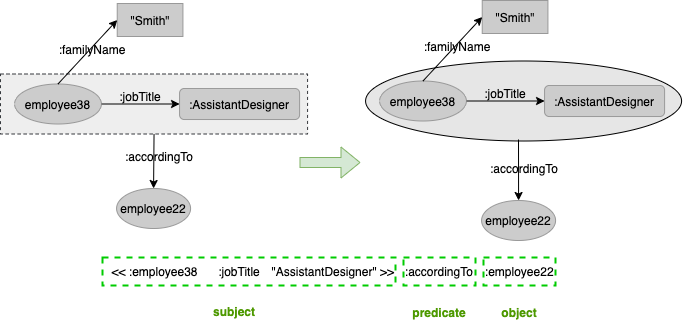
\includegraphics[scale=0.5]{images/Example-2-To-Nested.png}
    \end{figure}
\end{frame}

\begin{frame}[fragile]{Overview of the RDF-star Approach}{Nested triple patterns}
\vspace{2mm}
\begin{minipage}{0.8\textwidth}
SPARQL to the standard Reification:
\begin{lstlisting}[language=SPARQL,basicstyle=\ttfamily\footnotesize]
PREFIX ...
SELECT ?who ?whom WHERE {
 ?claim rdf:type rdf:Statement .
 ?claim rdf:subject ?who .
 ?claim rdf:predicate :jobTitle .
 ?claim rdf:object :AssistantDesigner .
 ?claim :accordingTo ?whom .
}
\end{lstlisting}
\end{minipage}
\begin{minipage}{0.8\textwidth}
\centering
\end{minipage}
\\SPARQL-Star over RDF-star is easier to query.
\begin{minipage}{0.8\textwidth}
\begin{lstlisting}[language=SPARQL,basicstyle=\ttfamily\footnotesize]
PREFIX ...
SELECT ?who ?whom WHERE {
 <<?who :jobTitle "AssistantDesigner">> :accordingTo ?claim .
 ?claim :accordingTo ?whom .
}
\end{lstlisting}
\end{minipage}
\end{frame}

\begin{frame}{Overview of the RDF-star Approach}{A brief history}

    \begin{itemize}
        \item April 2012, Dagstuhl seminar on Semantic Data Management
        \item Before 2013, an implementation in Blazegraph ("reification done right")
        \item June 2014, technical report that defines the RDF*/SPARQL* (Foundations of an Alternative Approach to Reification in RDF)
        \item Adoption in many systems:
            \begin{itemize}
                \item Blazegraph, AnzoGraph, Stardog, GraphDB, Neo4j neosemantics
                \item Apache Jena, Eclipse RDF4J, RDF.rb, N3.js, EYE
                \item YAGO 4 knowledge graph released as a Turtle* file
            \end{itemize}
        \item March 2019, W3C Workshop on Web Standardization for Graph Data in Berlin
        \item Community task force as part of the W3C RDF-DEV CG
            \begin{itemize}
                \item Mixture of implementer, users, and academic researchers
                \item Goal: create a spec that captures all aspects of the approach in the form of a CG report, plus a collection of corresponding test suites
                \item Some aspects of the approach have changed $\rightarrow$ new-names: RDF-star, SPARQL-star, etc.
            \end{itemize}
    \end{itemize}

\end{frame}

% \begin{frame}{Overview of the RDF-star Approach}{RDF-star and related specs}
    
% \end{frame}

% \begin{frame}{Overview of the RDF-star Approach}{Asserted Triples vs. Quoted Triples}
%     \begin{example}
%         \begin{itemize}
%             \item[] \texttt{PREFIX  : <http://www.example.org>}
%         	\item[] \texttt{:exployee38     :familyName   "Smith" .}
%         	\item[] \texttt{<< :employee38    :jobTitle   "AssistantDesigner" >> :accordingTo :employee22 .}
%         \end{itemize}
%     \end{example}
%     \begin{itemize}
%         \item Note: "employee38 has a jobTitle of Assistant Designer" is not an \textbf{asserted triple} but \textbf{quoted triple}.
%     \end{itemize}
% \end{frame}

% \begin{frame}{Overview of the RDF-star Approach}{Asserted Triples vs. Quoted Triples}
%     \begin{example}
%         \begin{itemize}
%             \item[] \texttt{PREFIX  : <http://www.example.org>}
%         	\item[] \texttt{:exployee38}
%         	\item[] \texttt{\quad :familyName   "Smith";}  
%         	\item[] \texttt{\quad :jobTitle   "Assistant Designer" \{| :accordingTo employee22|} \} .  
%         	\item[] \texttt{\# this is equivalent to: }  
%         	\item[] \texttt{\# :exployee38     :familyName   "Smith" .}
%         	\item[] \texttt{\# :employee38    :jobTitle   "AssistantDesigner" .}
%         	\item[] \texttt{\# << :employee38    :jobTitle   "AssistantDesigner" >> :accordingTo :employee22 .}
%         \end{itemize}
%     \end{example}
%     \begin{itemize}
%         \item Note: "employee38 has a jobTitle of Assistant Designer" is both an \textbf{asserted triple} and a \textbf{quoted triple}.
%     \end{itemize}
% \end{frame}

\section{Concepts and Abstract Syntax}
\begin{frame}{Concepts and Abstract Syntax}{RDF-star Data}
    \begin{itemize}
        \item \textbf{RDF-star graph}: a set of RDF-star triples
        \begin{itemize}
        \item Any RDF graph is a RDF-star graph
        \end{itemize}
        \item \textbf{RDF-star triple}: a 3-part tuple (subject, predicate, object)
        \begin{itemize}
            \item Any RDF triple is a RDF-star triple
            \item If $t$ and $t^{\prime}$ are RDF-star triples, $s$ is an IRI or a blank node, $p$ is an IRI, $o$ is an IRI, a blank node or literal, then ($t$, $p$, $o$), ($s$, $p$, $t$) and ($t$, $p$, $t^{\prime}$) are RDF-star triples
        \end{itemize}
        \item \textbf{RDF-star terms}: IRIs, literals, blank nodes and RDF-star triples
        \item \textbf{RDF-star dataset}: a collection of RDF-star graphs, and comprises
            \begin{itemize}
                \item Exactly one default graph
                \item Zero or more named graphs
                \item Any RDF dataset is also a RDF-star dataset
            \end{itemize}
    \end{itemize}
\end{frame}

\begin{frame}{Concepts and Abstract Syntax}{Asserted Triples vs. Quoted Triples}
    \begin{itemize}
        \item \textbf{Asserted triple}: RDF-star triple used as the subject or object of another RDF-star triple, also called \textbf{embedded triples}.
    \end{itemize}
    \begin{minipage}{\textwidth}
    \centering
    \textcolor{red}{:employee38 :familyName   "Smith" }
    \end{minipage}
    \begin{itemize}
        \item \textbf{Quoted triple}: RDF-star triple that is an element of a RDF-star graph (and they can be recursive)
    \end{itemize}
    \begin{minipage}{\textwidth}
    \centering
    \textcolor{red}{<<  :employee38 :jobTitle   "AssistantDesigner" >>}
    \end{minipage}
    Note: A quoted triple does not imply that it also exists as an asserted triple.\\
    Note on the note: An asserted triple (e.g. via annotation on the next slide) cannot be cancelled.

\end{frame}

\section{RDF-star Concrete Syntaxes}
\begin{frame}[fragile]{RDF-star Concrete Syntaxes}{Turtle-star}
\begin{itemize}
    \item An extension of the Turtle format for representing RDF-star graphs
    \item Replaces the production rules in the original grammar
    \item \textbf{Grammar}:
    \begin{itemize}
        \item \textcolor{red}{objectList}\quad\quad\quad::= \textcolor{blue}{\underline{object}} \textcolor{blue}{\textbf{\underline{annotation}}}\textcolor{red}{\textbf{?}} \textcolor{red}{\textbf{(}} \textcolor{gray}{','} \textcolor{blue}{\underline{object}} \textcolor{blue}{\textbf{\underline{annotation}}}\textcolor{red}{\textbf{?}} \textcolor{red}{\textbf{)*}}
        \item \textcolor{red}{subject}\quad::= iri \textcolor{red}{\textbf{|}} BlankNode \textcolor{red}{\textbf{|}} collection \textcolor{red}{\textbf{|}} \textcolor{blue}{\textbf{quotedTriple}}
        \item \textcolor{red}{object}\quad::= iri \textcolor{red}{\textbf{|}} BlankNode \textcolor{red}{\textbf{|}} collection \textcolor{red}{\textbf{|}} blankNodePropertyList \textcolor{red}{\textbf{|}} literal \textcolor{red}{\textbf{|}} \textcolor{blue}{\textbf{quotedTriple}}
        \item \textcolor{red}{\textbf{quotedTriple}}\quad::= \textcolor{gray}{'<<'} \textcolor{blue}{\textbf{qtSubject}} \textbf{verb} \textcolor{blue}{\textbf{qtObject}} \textcolor{gray}{'>>'}
        \item \textcolor{red}{\textbf{qtSubject}}\quad::= \textbf{iri} \textcolor{red}{\textbf{|}} \textbf{BlankNode} \textcolor{red}{\textbf{|}} \textcolor{blue}{\textbf{quotedTriple}}
        \item \textcolor{red}{\textbf{qtObject}}\quad::= \textbf{iri} \textcolor{red}{\textbf{|}} \textbf{BlankNode} \textcolor{red}{\textbf{|}} \textbf{literal} \textcolor{red}{\textbf{|}} \textcolor{blue}{\textbf{quotedTriple}}
        \item \textcolor{red}{\textbf{annoation}}\quad::= \textcolor{gray}{'\{|'} \textbf{predicateObjectList} \textcolor{gray}{'|\}'}
    \end{itemize}
\end{itemize}
\end{frame}

\begin{frame}[fragile]{RDF-star Concrete Syntaxes}{Turtle-star: A simple example}
    \begin{lstlisting}[language=TTL]
PREFIX : <http://www.example.org/>
:employee38 :familyName "Smith" .
<<:employee38 :jobTitle "AssistantDesigner">> :accordingTo :employee22 . 
    \end{lstlisting}
    versus
    \begin{lstlisting}[language=TTL]
PREFIX : <http://www.example.org/>
:employee38 :familyName "Smith" .
:employee38 :jobTitle "AssistantDesigner" .
<<:employee38 :jobTitle AssistantDesigner">> :accordingTo :employee22 . 
    \end{lstlisting}
\end{frame}

\begin{frame}[fragile]{RDF-star Concrete Syntaxes}{Turtle-star: Annotation Syntax}
    \begin{lstlisting}[language=TTL]
PREFIX : <http://www.example.org/>
:employee38 :jobTitle "AssistantDesigner" {| :accordingTo :employee22 |}. 
    \end{lstlisting}
    equals
    \begin{lstlisting}[language=TTL]
PREFIX : <http://www.example.org/>
<<:employee38 :jobTitle "AssistantDesigner">> :accordingTo :employee22. 
:employee38 :jobTitle "AssistantDesigner".
    \end{lstlisting}
    \begin{itemize}
        \item Annotation syntax does not appear in the RDF-star abstract data model $\rightarrow$ only a syntactic shortcut
        \item RDF-star abstract data model does not distinguish how the triples were written
    \end{itemize}
\end{frame}

\begin{frame}[fragile]{RDF-star Concrete Syntaxes}{Turtle-star: A more complex example}
    \begin{lstlisting}[language=TTL]
PREFIX : <http://www.example.org/>
:employee38 :familyName "Smith" .
:jobTitle   "AssistantDesigner" {| :accordingTo :employee22; 
                                    :startDate "2021-09-21"^^xsd:date |}. 
    \end{lstlisting}
    \begin{figure}
        \centering
        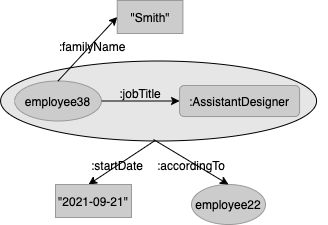
\includegraphics[scale=0.45]{images/Example-2-Turtle-start-Complex.png}
    \end{figure}
\end{frame}

\begin{frame}{RDF-star Concrete Syntaxes}{N-Triples-star}
    \begin{itemize}
        \item A minimal extension of the N-Triples format allowing a subject or an object of a RDF-star triple to be a quoted triple.
        \item No annotation syntax
        \item \textbf{Grammar}:
        \begin{itemize}
            \item \textcolor{red}{subject}\quad\quad\quad::= IRIREF | BLANK\_NODE\_LABEL | \textcolor{blue}{\textbf{quotedTriple}}
            \item \textcolor{red}{object}\quad\quad\quad::= IRIREF | BLANK\_NODE\_LABEL | literal | \textcolor{blue}{\textbf{quotedTriple}}
            \item \textcolor{red}{\textbf{quotedTriple}}\quad\quad\quad::= \textbf{"<<"} \textcolor{blue}{\textbf{\underline{subject}}} \textbf{predicate} \textcolor{blue}{\textbf{\underline{object}}} \textbf{">>"}
        \end{itemize}
    \end{itemize}
\end{frame}

\begin{frame}{RDF-star Concrete Syntaxes}{TriG-star}
    \begin{itemize}
        \item Minimal extension of the TriG format
        \item TriG-star document defines a RDF-star dataset, composed of a single default graph and zero or more named graphs, all of which are RDF-star graphs
        \item \textbf{Grammar}:
        \begin{itemize}
            \item \textcolor{red}{triplesOrGraph}\quad::= labelOrSubject \textcolor{red}{\textbf{(}} wrappedGraph \textcolor{red}{\textbf{|}} predicateObjectList \textcolor{red}{\textbf{'.')}} \textcolor{red}{\textbf{|}} \textcolor{blue}{\textbf{\underline{quotedTriple}}} \textbf{predicateObjectList} \textcolor{red}{\textbf{'.'}}
            \item \textcolor{red}{objectList}\quad\quad\quad::= \textcolor{blue}{\underline{object}} \textcolor{blue}{\textbf{\underline{annotation}}}\textcolor{red}{\textbf{?}} \textcolor{red}{\textbf{(}} \textcolor{gray}{','} \textcolor{blue}{\underline{object}} \textcolor{blue}{\textbf{\underline{annotation}}}\textcolor{red}{\textbf{?}} \textcolor{red}{\textbf{)*}}
            \item \textcolor{red}{subject}\quad::= iri \textcolor{red}{\textbf{|}} BlankNode \textcolor{red}{\textbf{|}} collection \textcolor{red}{\textbf{|}} \textcolor{blue}{\textbf{quotedTriple}}
            \item \textcolor{red}{object}\quad::= iri \textcolor{red}{\textbf{|}} BlankNode \textcolor{red}{\textbf{|}} collection \textcolor{red}{\textbf{|}} blankNodePropertyList \textcolor{red}{\textbf{|}} literal \textcolor{red}{\textbf{|}} \textcolor{blue}{\textbf{quotedTriple}}
            \item \textcolor{red}{\textbf{quotedTriple}}\quad::= \textcolor{gray}{'<<'} \textcolor{blue}{\textbf{qtSubject}} \textbf{verb} \textcolor{blue}{\textbf{qtObject}} \textcolor{gray}{'>>'}
            \item \textcolor{red}{\textbf{qtSubject}}\quad::= \textbf{iri} \textcolor{red}{\textbf{|}} \textbf{BlankNode} \textcolor{red}{\textbf{|}} \textcolor{blue}{\textbf{quotedTriple}}
            \item \textcolor{red}{\textbf{qtObject}}\quad::= \textbf{iri} \textcolor{red}{\textbf{|}} \textbf{BlankNode} \textcolor{red}{\textbf{|}} \textbf{literal} \textcolor{red}{\textbf{|}} \textcolor{blue}{\textbf{quotedTriple}}
            \item \textcolor{red}{\textbf{annoation}}\quad::= \textcolor{gray}{'\{|'} \textbf{predicateObjectList} \textcolor{gray}{'|\}'}
        \end{itemize}
    \end{itemize}
\end{frame}


\begin{frame}{RDF-star Concrete Syntaxes}{Other concrete syntaxes}
    \begin{itemize}
        \item N-Quads-star
        \begin{itemize}
            \item For RDF-star datasets
            \item N-Triples-star + optional graph name
        \end{itemize}
        \item JSON-LD-star
        \begin{itemize}
            \item https://json-ld.github.io/json-ld-star/
        \end{itemize}
    \end{itemize}
\end{frame}

\section{SPARQL-star Query Language}
\begin{frame}{SPARQL-star Query Language}{Definitions}
    \begin{itemize}
        \item A \textbf{SPARQL-star triple pattern} is a 3-tuple defined recursively as follows:
        \begin{itemize}
            \item Every SPARQL triple pattern is a SPARQL-star triple pattern
            \item If $t$ and $t^{\prime}$ are SPARQL-star triple patterns, $x$ is an RDF term or a query variable, and $p$ is an IRI or a query variable, then ($t$, $p$, $x$), ($x$, $p$, $t$), and ($t$, $p$, $t^{\prime}$) are SPARQL-star triple patterns
        \end{itemize}
        \item A \textbf{SPARQL-star basic graph pattern} (BGP-star) is a set of SPARQL-star triple patterns
        \item A \textbf{SPARQL-star property path pattern} is a 3-tuple ($s$, $p$, $o$) where
            \begin{itemize}
                \item $s$ is either a RDF term, a query variable, or a SPARQL-star triple pattern
                \item $p$ is a property path expression, and
                \item $o$ is either a RDF term, a query variable, or a SPARQL-star triple pattern
            \end{itemize}
            \item A \textbf{SPARQL-star solution mapping} $\mu$ is a partial function from the set of all query variables to the set of all RDF-star terms. The domain of $\mu$ is the set of query variable for which $\mu$ is defined
    \end{itemize}
\end{frame}

\begin{frame}{SPARQL-star Query Language}{Grammar}
    SPARQL-star is defined to follow the same grammar as SPARQL 1.1, except for the EBNF productions (not complete) specified below.
    \begin{itemize}
        \item \textcolor{red}{Object}\quad::= \textcolor{blue}{GraphNode} \textcolor{blue}{\textbf{AnnotationPattern}}\textcolor{red}{\textbf{?}}
        \item \textcolor{red}{ObjectPath}\quad::= \textcolor{blue}{GraphNodePath} \textcolor{blue}{\textbf{AnnotationPatternPath}}\textcolor{red}{\textbf{?}}
        \item \textcolor{red}{GraphNode}\quad::= \textcolor{blue}{\textbf{VarOrTermOrEmbTP}} \textcolor{red}{\textbf{|}} \textcolor{blue}{TriplesNode}
        \item \textcolor{red}{GraphNodePath}\quad::= \textcolor{blue}{\textbf{VarOrTermOrEmbTP}} \textcolor{red}{\textbf{|}} \textcolor{blue}{TriplesNodePath}
        \item \textcolor{red}{\textbf{EmbTP}}\quad\quad\quad::= \textbf{'<<'} \textcolor{blue}{\textbf{\underline{EmbSubjectOrObject}}} \textbf{\underline{Verb}} \textcolor{blue}{\textbf{\underline{EmbSubjectOrObject}}} \textbf{'>>'}
        \item \textcolor{red}{\textbf{EmbTriple}}\quad\quad\quad::= \textbf{'<<'} \textcolor{blue}{\textbf{\underline{DataValueTerm}}} \textcolor{red}{\textbf{(}} \textcolor{blue}{\underline{iri}} \textcolor{red}{\textbf{|}} \textcolor{gray}{\textbf{'a'}} \textcolor{red}{\textbf{)}} \textcolor{blue}{\textbf{\underline{DataValueTerm}}} \textbf{'>>'}
        \item \textcolor{red}{\textbf{VarOrTermOrEmbTP}}\quad\quad\quad::= \textcolor{blue}{\underline{\textbf{Var}}} \textcolor{red}{\textbf{|}} \textcolor{blue}{\underline{\textbf{GraphTerm}}} \textcolor{red}{\textbf{|}} \textcolor{blue}{\textbf{\underline{EmbTP}}}
    \end{itemize}
\end{frame}

\begin{frame}{SPARQL-star Query Language}{Translation to the Algebra (1/7)}
    \begin{itemize}
        \item SPARQL specification defines a process based on the SPARQL grammar, to convert graph patterns and solution modifiers in a SPARQL query string into a SPARQL algebra expression
        \item[$\Rightarrow$] Must be adjusted to the extended grammar
        \item Here: Only discussion of steps which require adjustment
    \end{itemize}
\end{frame}

\begin{frame}{SPARQL-star Query Language}{Translation to the Algebra (2/7)}
    \begin{itemize}
        \item \textbf{Expand variable scope}
            \begin{itemize}
                \item A variable is in-scope of a BGQ-star \textit{B} if the variable occurs in \textit{B}, which includes an occurence in any embedded triple pattern in \textit{B} (independent of the level of nesting)
                \item A variable is in-scope of a property path pattern if the variable occurs in that pattern, which includes an occurence in any embedded triple pattern in the pattern (independent of the level of nesting)
            \end{itemize}
    \end{itemize}
\end{frame}

\begin{frame}[fragile]{SPARQL-star Query Language}{Translation to the Algebra (3/7)}
    \begin{itemize}
        \item \textbf{Expand Syntax Forms}
            \begin{itemize}
                \item Annotation patterns \textbf{MUST} be replaced by additional SPARQL-star triple pattern that have the annotated triple pattern as an embedded triple pattern in their subject position
            \end{itemize}
    \end{itemize}
    \begin{lstlisting}[language=TTL]
?x :p :o1 {| :ap1 ?y;
             :ap2 ?z |} ,
      :o2 {| :ap3 ?z |} .
?x :p :o3 {| :ap4/:ap5 ?w } .
    \end{lstlisting}
    $\Rightarrow$\textcolor{red}{must be replaced by}
    \begin{lstlisting}[language=TTL ]
?x :p :o1, o2 .
<<?x :p :o1>> :ap1 ?y ;
              :ap2 ?z .
<<?x :p :o2>> :ap3 ?z .
?x :p :o3 .
<<?x :p :o3>> :ap4/:ap5 ?w .
    \end{lstlisting}
\end{frame}

\begin{frame}[fragile]{SPARQL-star Query Language}{Translation to the Algebra (4/7)}
    \begin{itemize}
        \item \textbf{Expand Syntax Forms}
            \begin{itemize}
                \item Abbreviations for triple patterns with embedded triple patterns \textbf{MUST} be expanded as if each embedded triple pattern was a variable (or a RDF-term).
            \end{itemize}
    \end{itemize}
                    \begin{lstlisting}[language=TTL ]
<<?c a owl:Class>> dct:source ?src ;
                  :entailing <<?c a rdfs:Class>> .
                \end{lstlisting}
                $\Rightarrow$ \textcolor{red}{must be expanded to}
                    \begin{lstlisting}[language=TTL ]
<<?c a owl:Class>> dct:source ?src .
<<?c a owl:Class>> :entailing <<?c a rdfs:Class>> .
                \end{lstlisting}
\end{frame}

\begin{frame}[fragile]{SPARQL-star Query Language}{Translation to the Algebra (5/7)}
    \begin{itemize}
        \item \textbf{Expand Syntax Forms}
            \begin{itemize}
                \item Abbreviations for IRIs in all embedded triple patterns MUST be expanded.
            \end{itemize}
    \end{itemize}
\begin{lstlisting}[language=TTL ]
<<?c a rdfs:Class>>
\end{lstlisting}
   $\Rightarrow$ \textcolor{red}{must be expanded to}
\begin{lstlisting}[language=TTL ]
<< ?c <http://www.w3.org/1999/02/22-rdf-syntax-ns#type>
                <http://www.w3.org/2000/01/rdf-schema#Class>>>
\end{lstlisting}
\end{frame}

\begin{frame}{SPARQL-star Query Language}{Translation to the Algebra (6/7)}
    \begin{itemize}
        \item \textbf{Translate Property Path Patterns}
        \begin{itemize}
            \item Let \textit{X} \textit{P} \textit{Y} be a string where \textit{X} and \textit{Y} may be a RDF term, or an embedded triple pattern, respectively, and \textit{P} is a property path expression (see also \url{https://www.w3.org/TR/sparql11-query/\#sparqlTranslatePathPatterns})
            \item The string \textit{X} \textit{P} \textit{Y} is translated to the algebra expression Path(\textit{X}$^{\prime}$, \textit{P}, \textit{Y}$^\prime$) as the result of calling a function named Lift for \textit{X} and \textit{Y}, respectively
        \end{itemize}
    \end{itemize}
    \begin{block}{Lift}
    For some input string \textit{Z} that can be a RDF term, a variable, or an embedded triple pattern, the function \textbf{Lift} is defined recursively as follows:
    \begin{enumerate}
        \item If \textit{Z} is an embedded triple pattern <<S, P, O>> then return the SPARQL-star triple pattern (Lift(S), P, Lift(O));
        \item Otherwise, return \textit{Z}.
    \end{enumerate}
    \end{block}
\end{frame}

\begin{frame}{SPARQL-star Query Language}{Translation to the Algebra (7/7)}
    \begin{itemize}
        \item \textbf{Translate Basic Graph Patterns}
        \begin{itemize}
            \item Triple patterns in the extended syntax may have an embedded triple pattern in their subject position or in their object position (or both).
            \item To ensure that every result of this step is a BGP-star, before adding a triple pattern to its corresponding collection, its subject and object \textbf{MUST} be replaced by the result of calling function Lift for the subject and the object, respectively
        \end{itemize}
    \end{itemize}
\end{frame}

\begin{frame}{SPARQL-star Query Language}{New Built-In Function and Operator Definitions}
\begin{itemize}
    \item \textbf{TRIPLE}
    \item[] \textcolor{red}{RDF-star triple} \textbf{TRIPLE} (\textcolor{red}{RDF-star term} term1, \textcolor{red}{RDF-star term} term2, \textcolor{red}{RDF-star term} term3)
    \item \textbf{SUBJECT}
    \item[] \textcolor{red}{RDF-star term} \textbf{SUBJECT} ( \textcolor{red}{RDF-star triple} triple )
    \item \textbf{PREDICATE}
    \item[] \textcolor{red}{RDF-star term} \textbf{PREDICATE} ( \textcolor{red}{RDF-star triple} triple )
    \item \textbf{OBJECT}
    \item[] \textcolor{red}{RDF-star term} \textbf{OBJECT} ( \textcolor{red}{RDF-star triple} triple )
    \item \textbf{isTRIPLE}
    \item[] \textcolor{red}{xsd:boolean} \textbf{isTRIPLE} ( \textcolor{red}{RDF-star term} term )
\end{itemize}
\end{frame}

\begin{frame}[fragile]{SPARQL-star Query Language}{New Built-In Function and Operator Definitions}
Examples:
\begin{lstlisting}[language=SPARQL]
SELECT ?cartoon ?y ?o
WHERE {
    ?cartoon :depicts << :bob :dreamingOf ?y>>
    FILTER (isTriple(?y))
    BIND (Object(?y) AS ?o)
}
\end{lstlisting}

\begin{lstlisting}[language=SPARQL]
SELECT ?cartoon ?t
WHERE {
    ?cartoon :depicts << ?x :dreamingOf ?y>>
    BIND (TRIPLE (?x,:state,:sleeping) AS ?t)
}
\end{lstlisting}
\end{frame}

\begin{frame}{SPARQL-star Query Language}{New Built-In Function and Operator Definitions}
\begin{itemize}
    \item \textbf{Embedded Triple Expression}
    \item[] \textcolor{red}{RDF-star triple} \textbf{<<} (\textcolor{red}{RDF-star term} term1, \textcolor{red}{RDF-star term} term2, \textcolor{red}{RDF-star term} term3 \textbf{>>}
    \item \textbf{sameTerm}
    \item[] \textcolor{red}{xsd:boolean} \textbf{sameTerm} (term, term)
    \item \textbf{sparql-compare}
    \item[] \textcolor{red}{xsd:boolean} \textbf{sparql-compare} ( RDF-star term, RDF-star term )
    \item \textbf{RDFterm-equal}
    \item[] The function is the default dispatch for the \textcolor{red}{=} operator.
\end{itemize}
\end{frame}

\begin{frame}{SPARQL-star Query Language}{Function and Operator Definitions}
\textbf{Definition: sparql-compare}
\begin{itemize}
    \item If neither A nor B is an RDF-star triple term, compare by SPARQL 1.1 operators <, =, >, ) and (, return the comparison value (-1, 0, +1) or throw an error as defined by SPARQL 1.1.
    \item If either A or B is an RDF-star triple term, and the other is not an RDF-star triple term, then error.
    \item If sparql-compare(SUBJECT(A), SUBJECT(B)) != 0, then return this value.
    \item If sparql-compare(PREDICATE(A), PREDICATE(B)) != 0, then return this value.
    \item Return sparql-compare(OBJECT(A), OBJECT(B))
\end{itemize}
\end{frame}

\begin{frame}{SPARQL-star Query Language}{Function and Operator Definitions}
\begin{itemize}
    \item \textbf{Operator Mappings}
    \begin{figure}
        \centering
        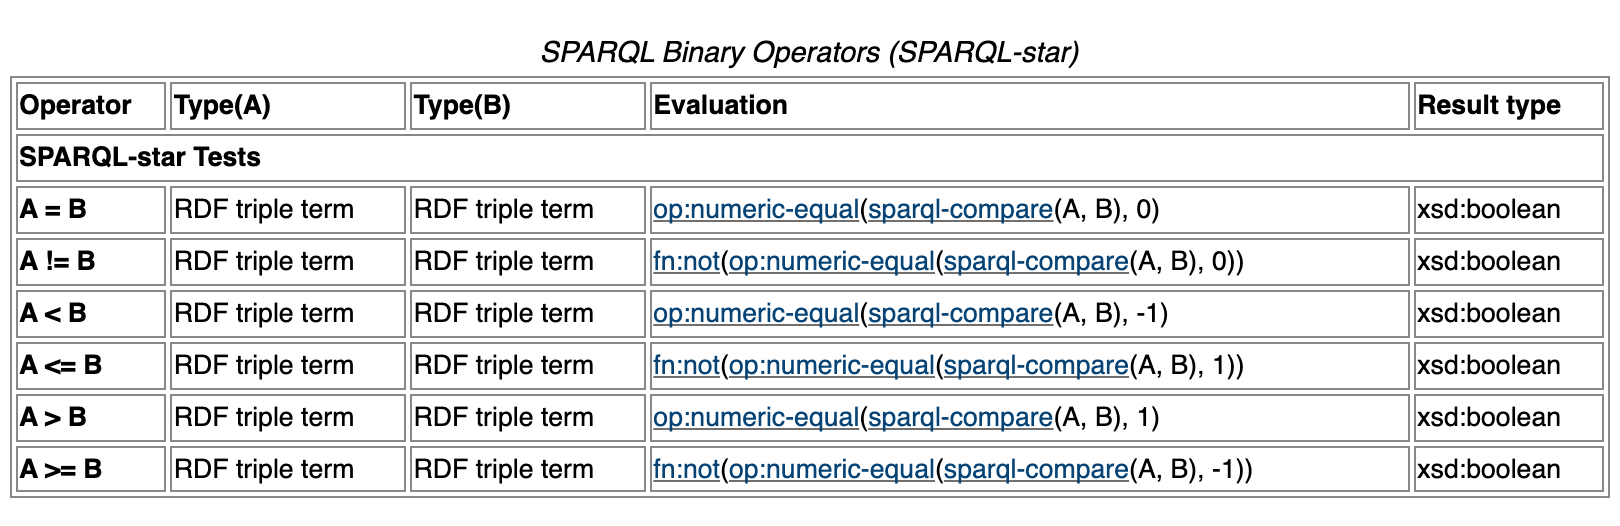
\includegraphics[scale=0.5]{images/SPARQL Binary Operators (SPARQL-star).png}
        \caption{Source: \url{https://w3c.github.io/rdf-star/cg-spec/2021-07-01.html}}
    \end{figure}
\end{itemize}
\end{frame}

\begin{frame}{SPARQL-star Query Language}{Function and Operator Definitions}
\begin{itemize}
    \item \textbf{Triple term with ORDER BY}
    \begin{itemize}
        \item (Lowest) no value assigned to the variable or expression in this solution.
        \item Blank nodes
        \item IRIs
        \item RDF literals
        \item RDF-star triple terms
    \end{itemize}
\end{itemize}
\end{frame}

\begin{frame}[fragile]{SPARQL-star Query Language}{Query Result Formats}
\textbf{SPARQL-star Query Results JSON Format}
        Consider the following RDF term, an embedded triple in Turtle-star syntax:
\begin{lstlisting}[language=TTL ]
<< <http://example.org/alice> <http://example.org/name> "Alice" >>}}
\end{lstlisting}
        This term is represented in JSON as follows:
\begin{lstlisting}[language=JSON, numbers=none,  basicstyle=\tiny, ]
 {"type": "triple",
  "value": {
    "subject": {
        "type": "uri",
        "value" "http://example.org/alice"
    },
    "predicate": {
        "type": "uri",
        "value" "http://example.org/name"
    },
 "object": {
 "type": "literal",
 "value" "Alice",
 "datatype": "http://www.w3.org/2001/XMLSchema#string"},
}}
\end{lstlisting}
\end{frame}

\begin{frame}[fragile]{SPARQL-star Query Language}{Query Result Formats}
\textbf{SPARQL-star Query Results XML Format}
        Consider the following RDF term, an embedded triple in Turtle-star syntax:
\begin{lstlisting}[language=TTL ]
<< <http://example.org/alice> <http://example.org/name> "Alice" >>}}
\end{lstlisting}
        This term is represented in XML as follows:
\begin{lstlisting}[language=JSON, numbers=none,  basicstyle=\scriptsize, showspaces=false,  showstringspaces=false,  showtabs=false,   ]
<triple>
    <subject>
        <uri>http://example.org/alice</uri>
    </subject>
    <predicate>
        <uri>http://example.org/name</uri>
    </predicate>
    <object>
        <literal datatype='http://www.w3.org/2001/XMLSchema#string'>Alice</literal>
    </object>
</triple>
\end{lstlisting}
 
\end{frame}

\begin{frame}[fragile]{SPARQL-star Query Language}{SPARQL-star Update}
INSERT DATA
 
\begin{lstlisting}[language=SPARQL]
PREFIX : <http://www.example.org/>
INSERT DATA {
    :alice :claims << :bob :age 23 >> .
}
\end{lstlisting}
\begin{lstlisting}[language=SPARQL]
PREFIX : <http://www.example.org/>
INSERT DATA {
    :bob :age 23 .
    :alice :claims << :bob :age 23 >> .
}
\end{lstlisting}
\end{frame}

\begin{frame}[fragile]{SPARQL-star Query Language}{SPARQL-star Update}
 DELETE DATA
\begin{lstlisting}[language=SPARQL]
PREFIX : <http://www.example.org/>
DELETE DATA {
    :alice :claims << :bob :age 23 >> .
}
\end{lstlisting}
\begin{lstlisting}[language=SPARQL]
PREFIX : <http://www.example.org/>
DELETE DATA {
    :bob :age 23 .
}
\end{lstlisting}
\end{frame}

\begin{frame}[fragile]{SPARQL-star Query Language}{SPARQL-star Update}
DELETE/INSERT
\begin{lstlisting}[language=SPARQL]
PREFIX : <http://www.example.org/>
DELETE { :alice ?pp <<?s ?p ?o>> . }
INSERT { :carol ?pp <<?s ?p ?o>> . }
WHERE {  :alice ?pp <<?s ?p ?o>> . }
\end{lstlisting}
\begin{lstlisting}[language=SPARQL]
PREFIX : <http://www.example.org/>
DELETE { :alice ?pp <<?s ?p ?o>> . }
INSERT { :carol ?pp <<?s ?p ?o>> .  ?s ?p ?o .}
WHERE {  :alice ?pp <<?s ?p ?o>> . }
\end{lstlisting}
\end{frame}

\begin{frame}[fragile]{SPARQL-star Query Language}{SPARQL-star Update}
 DELETE/INSERT
\begin{lstlisting}[language=SPARQL]
PREFIX : <http://www.example.org/>
INSERT {
    GRAPH :graph2 { ?s ?p ?o }
}
WHERE {
    { <<?s ?p ?o>> ?pp ?oo }
    UNION
    { ?ss ?pp <<?s ?p ?o>> }    
}
\end{lstlisting}
\end{frame}

\section{Use Cases and Current Discussions}
\begin{frame}{Use Cases}
 \begin{itemize}
     \item Use Cases for justification are collected \url{https://w3c.github.io/rdf-star/UCR/rdf-star-ucr.html}
     \item Still an active field of discussion \url{https://lists.w3.org/Archives/Public/public-rdf-star/2021Dec/0001.html}
     \item (Strongly disputed) Use case by Amazon \url{https://lists.w3.org/Archives/Public/public-rdf-star/2021Dec/att-0001/rdf-star-neptune-use-cases-20211202.pdf} $\rightarrow$ We are still not able to model every real-world use case with satisfaction
 \end{itemize}

\end{frame}

\begin{frame}{Summary}{Outlook}
	\begin{itemize}
	    \item 2nd community report underway \url{https://w3c.github.io/rdf-star/cg-spec/editors_draft.html}
		\item SHACL-star as another extension
		\item W3C Recommendation Track for the Community Group
\end{itemize}
\end{frame}

\begin{frame}{Summary}{References}
	\begin{itemize}
		\item Olaf Hartig, Pierre-Antoine, Gregg Kellogg, and Andy Seaborne. \\ RDF-star and SPARQL-star, Draft Community Group Report, \url{https://w3c.github.io/rdf-star/cg-spec/2021-07-01.html}, 01 July 2021.
		\item Richard Cyganiak, David Wood, and Markus Lanthaler. RDF 1.1 Concepts and Abstract Syntax, \url{https://www.w3.org/TR/rdf11-concepts/}, W3C Recommendation, 25 February 2014.
		\item Steve Harris, Andy Seaborne. SPARQL 1.1 Query Language, \url{https://www.w3.org/TR/sparql11-query/}. W3C Recommendation, 21 March 2013.
		\item \url{https://github.com/semantic-systems/rdf-star-tutorial} Simple tutorial 
		\item \url{http://www.lotico.com/index.php/Metadata_for_RDF_Statements:_The_RDF-star_Approach} Video lecture by Olaf Hartig and Pierre-Antoine Champin
\end{itemize}
\end{frame}

\end{document}